\pdfminorversion=7
\documentclass{beamer}
\usetheme{Boadilla}

\usepackage[T2A]{fontenc}
\usepackage[utf8]{inputenc}
\usepackage[english,russian]{babel}
\usepackage{amsmath,amssymb}
\usepackage{array}
\usepackage{booktabs}
\usepackage{graphicx}
\usepackage{pdfpages}
\usepackage{ragged2e}
\usepackage{tikz}
\usetikzlibrary{arrows.meta,positioning}

\graphicspath{{./images/}{./images/logo/}{./extra/}}

\setbeamertemplate{navigation symbols}{}
\setbeamertemplate{caption}[numbered]
\setbeamerfont{frametitle}{size=\large}
\setbeamerfont{caption}{size=\scriptsize}
\setbeamersize{text margin left=7mm,text margin right=7mm}

\newcommand{\jj}{\righthyphenmin=20\justifying}
\newcommand{\smallitem}{\setlength{\itemsep}{0.35em}}
\newcommand{\metric}[2]{\textbf{#1}\\{\scriptsize #2}}
\newcolumntype{L}[1]{>{\raggedright\arraybackslash}p{#1}}
\newcolumntype{C}[1]{>{\centering\arraybackslash}p{#1}}

\begin{document}

\begin{frame}[plain]
  \centering
  
\includegraphics[page=1,width=\textwidth,height=0.96\paperheight,keepaspectratio]{extra/tytle_presentation.pdf}
\end{frame}

\begin{frame}{Актуальность темы}
  \footnotesize
  \begin{columns}[T,onlytextwidth]
    \begin{column}{0.58\linewidth}
      \begin{itemize}
        \smallitem
        \item Цифровые активы граждан включают электронные документы, аккаунты, цифровые архивы, криптоактивы, цифровые права и иные объекты, имеющие имущественную, личную или доказательную ценность.
        \item После смерти владельца такие активы часто остаются вне наследственной процедуры: наследники могут не знать об их существовании, а платформы действуют по собственным правилам.
        \item Для нотариата важны проверяемые сведения о составе цифрового наследства, воле владельца и допустимом объёме раскрытия данных.
      \end{itemize}
    \end{column}
    \begin{column}{0.39\linewidth}
      \begin{block}{Проблема}
        Нет единого доверенного механизма, который связывает волю гражданина, нотариальную процедуру, государственные реестры и защищённое обращение с цифровыми активами.
      \end{block}
    \end{column}
  \end{columns}
\end{frame}

\begin{frame}{Цель, объект и предмет}
  \footnotesize
  \begin{block}{Цель работы}
    Разработка требований и концептуального проектного решения для государственной информационной системы управления, каталогизации и хранения цифровых активов граждан Российской Федерации с учётом правовых, организационных и экономических аспектов внедрения.
  \end{block}

  \begin{columns}[T,onlytextwidth]
    \begin{column}{0.48\linewidth}
      \begin{block}{Объект исследования}
        Деятельность Федеральной нотариальной палаты Российской Федерации.
      \end{block}
    \end{column}
    \begin{column}{0.48\linewidth}
      \begin{block}{Предмет исследования}
        Совокупность требований к системе управления цифровыми активами с учётом нормативно-правовой базы и современного уровня развития технологий.
      \end{block}
    \end{column}
  \end{columns}
\end{frame}

\begin{frame}{Задачи работы}
  \footnotesize
  \begin{enumerate}
    \smallitem
    \item Исследовать теоретические, правовые и методические основы управления цифровыми активами граждан, выявить проблемы и риски их хранения, передачи и наследования.
    \item Проанализировать существующие подходы, решения и институциональную среду, определить участников процесса и сформировать функциональные и нефункциональные требования к системе.
    \item Разработать концептуальное проектное решение государственной информационной системы и оценить экономическую эффективность её разработки и внедрения.
  \end{enumerate}

  \vspace{0.35cm}
  \begin{block}{Логика исследования}
    Методичка требует связи цели, задач, структуры работы и итоговых выводов; поэтому каждая задача соответствует одной главе ВКР и одному блоку результатов защиты.
  \end{block}
\end{frame}

\begin{frame}{Классификация цифровых активов}
  \tiny
  \renewcommand{\arraystretch}{0.95}
  \begin{table}
    \centering
    \begin{tabular}{L{0.19\linewidth} L{0.22\linewidth} L{0.18\linewidth} L{0.23\linewidth}}
      \toprule
      \textbf{Класс актива} & \textbf{Примеры} & \textbf{Ценность} & \textbf{Ключевой риск} \\
      \midrule
      Коммуникации и личные архивы & email, мессенджеры, фото, заметки & личная, доказательная & раскрытие частной жизни и данных третьих лиц \\
      Социальные сети и цифровой профиль & посты, профиль, социальный граф & мемориальная, репутационная & конфликт воли владельца, наследников и правил платформы \\
      Финансовые цифровые активы & банковские и брокерские счета, кошельки, криптоактивы & имущественная & потеря доступа, ошибочная или незаконная передача \\
      Гибридные активы & аккаунты с монетизацией, игровые и виртуальные объекты & финансовая + личная & смешение прав на аккаунт, контент и доходы \\
      \bottomrule
    \end{tabular}
  \end{table}

  \vspace{-0.05cm}
  \textbf{Вывод для проектирования:} система должна учитывать правовую природу, чувствительность, ликвидность, способ хранения и допустимые посмертные операции по активу.
\end{frame}

\begin{frame}{Масштаб цифровой среды}
  \begin{figure}
    \centering
    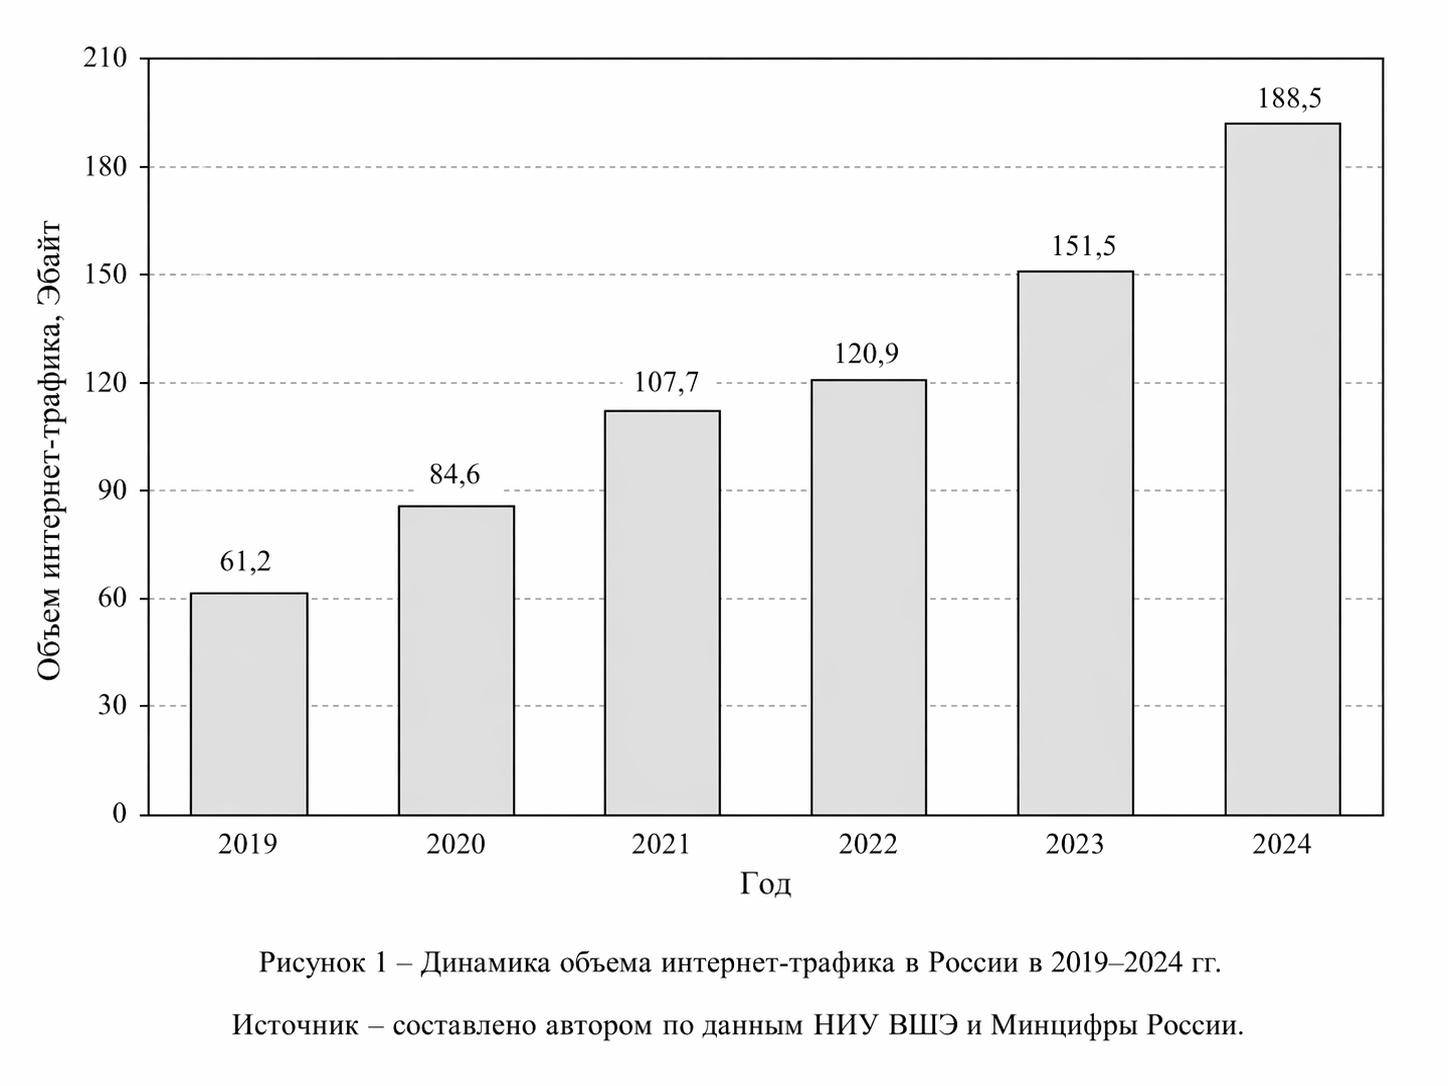
\includegraphics[width=0.66\linewidth,trim=0 145 0 0,clip]{internet_statistics.png}
    \caption{Динамика объёма интернет-трафика в России в 2019--2024 гг.}
  \end{figure}
\end{frame}

\begin{frame}{Риски управления цифровыми активами}
  \scriptsize
  \centering
  \resizebox{0.62\linewidth}{!}{%
  \begin{tikzpicture}[
      every node/.style={font=\small},
      main/.style={circle, draw, thick, minimum size=3.2cm, align=center},
      sector/.style={draw, thick, rounded corners, align=center, text width=3.9cm, inner sep=6pt},
      arrow/.style={-{Latex[length=3mm]}, thick}
  ]
    \node[main] (core) {Цифровые\\активы\\гражданина};
    \node[sector, above=2.65cm of core] (tech) {\textbf{Технические риски}\\T1 Потеря доступа\\T2 Компрометация\\T3 Долговременное хранение};
    \node[sector, right=4.2cm of core] (legal) {\textbf{Правовые риски}\\L1 Неопределённость статуса\\L2 Юрисдикции\\L3 Наследственные споры};
    \node[sector, below=2.65cm of core] (privacy) {\textbf{Конфиденциальность}\\P1 Тайна переписки\\P2 Репутационные риски\\P3 Права третьих лиц};
    \node[sector, left=4.2cm of core] (org) {\textbf{Организационные риски}\\O1 Отсутствие процессов\\O2 Человеческий фактор\\O3 Злоупотребления};
    \node[sector, above left=2.35cm and 3.05cm of core] (ethics) {\textbf{Этические риски}\\E1 Несоответствие воли\\E2 Конфликт ценностей};
    \draw[arrow] (tech) -- (core);
    \draw[arrow] (legal) -- (core);
    \draw[arrow] (privacy) -- (core);
    \draw[arrow] (org) -- (core);
    \draw[arrow] (ethics) -- (core);
  \end{tikzpicture}}

  \vspace{0.05cm}
  \begin{block}{Проектный принцип}
    Доступ должен быть минимально необходимым: участник получает только те сведения, которые соответствуют роли, правовому основанию, статусу наследственного дела и воле владельца.
  \end{block}
\end{frame}

\begin{frame}{Существующие решения и разрыв}
  \footnotesize
  \begin{columns}[T,onlytextwidth]
    \begin{column}{0.48\linewidth}
      \textbf{Что уже существует}
      \begin{itemize}
        \smallitem
        \item DAM, ECM/DMS, MAM, DRM/IAM-системы;
        \item электронные сервисы нотариата;
        \item механизмы Google, Apple, Microsoft и специализированные сервисы цифрового наследства.
      \end{itemize}
    \end{column}
    \begin{column}{0.48\linewidth}
      \textbf{Чего не хватает}
      \begin{itemize}
        \smallitem
        \item проверки юридически значимого события;
        \item связи с нотариальной процедурой и государственными реестрами;
        \item юридически значимого журналирования;
        \item долгосрочного хранения и контролируемого раскрытия сведений.
      \end{itemize}
    \end{column}
  \end{columns}

  \vspace{0.2cm}
  \begin{block}{Позиция работы}
    Требуется не хранилище паролей, а доверенный государственный информационный слой, встроенный в наследственный контур.
  \end{block}
\end{frame}

\begin{frame}{Участники и контуры системы}
  \scriptsize
  \begin{columns}[T,onlytextwidth]
    \begin{column}{0.48\linewidth}
      \textbf{Ключевые участники}
      \begin{itemize}
        \smallitem
        \item гражданин;
        \item наследник;
        \item доверенное лицо;
        \item нотариус;
        \item оператор системы;
        \item поставщики цифровых услуг;
        \item государственные реестры;
        \item публично-правовое образование.
      \end{itemize}
    \end{column}
    \begin{column}{0.48\linewidth}
      \textbf{Основные контуры}
      \begin{itemize}
        \smallitem
        \item пользовательский контур;
        \item контур нотариальной инфраструктуры;
        \item контур оператора и поставщиков услуг;
        \item контур государственных реестров и межведомственного обмена.
      \end{itemize}
    \end{column}
  \end{columns}
\end{frame}

\begin{frame}{Целевой процесс}
  \begin{figure}
    \centering
    
\includegraphics[width=\linewidth,height=0.78\textheight,keepaspectratio,trim=0 0 0 42,clip]{process_diagram.png}
    \caption{Сценарий взаимодействия участников в рамках наследственной процедуры}
  \end{figure}
\end{frame}

\begin{frame}{Группы требований к системе}
  \scriptsize
  \begin{table}
    \centering
    \begin{tabular}{L{0.26\linewidth} L{0.63\linewidth}}
      \toprule
      \textbf{Группа требований} & \textbf{Содержание} \\
      \midrule
      Идентификация и роли & ЕСИА, роли гражданина, наследника, доверенного лица, нотариуса, оператора и внешнего участника; многофакторная аутентификация для критических операций. \\
      Реестр цифровых активов & карточки активов, классификация, статусы, документы-основания, история изменений. \\
      Распоряжения владельца & наследники, доверенные лица, условия раскрытия, сценарии удаления, мемориализации, передачи или ограничения доступа. \\
      Защищённое хранение & гибридная модель: базовое хранение метаданных и расширенное хранение секретов после клиентского шифрования. \\
      Интеграция и аудит & нотариальная инфраструктура, государственные реестры, внешние платформы, журналирование юридически значимых действий. \\
      \bottomrule
    \end{tabular}
  \end{table}
\end{frame}

\begin{frame}{Архитектура проектного решения}
  \begin{figure}
    \centering
    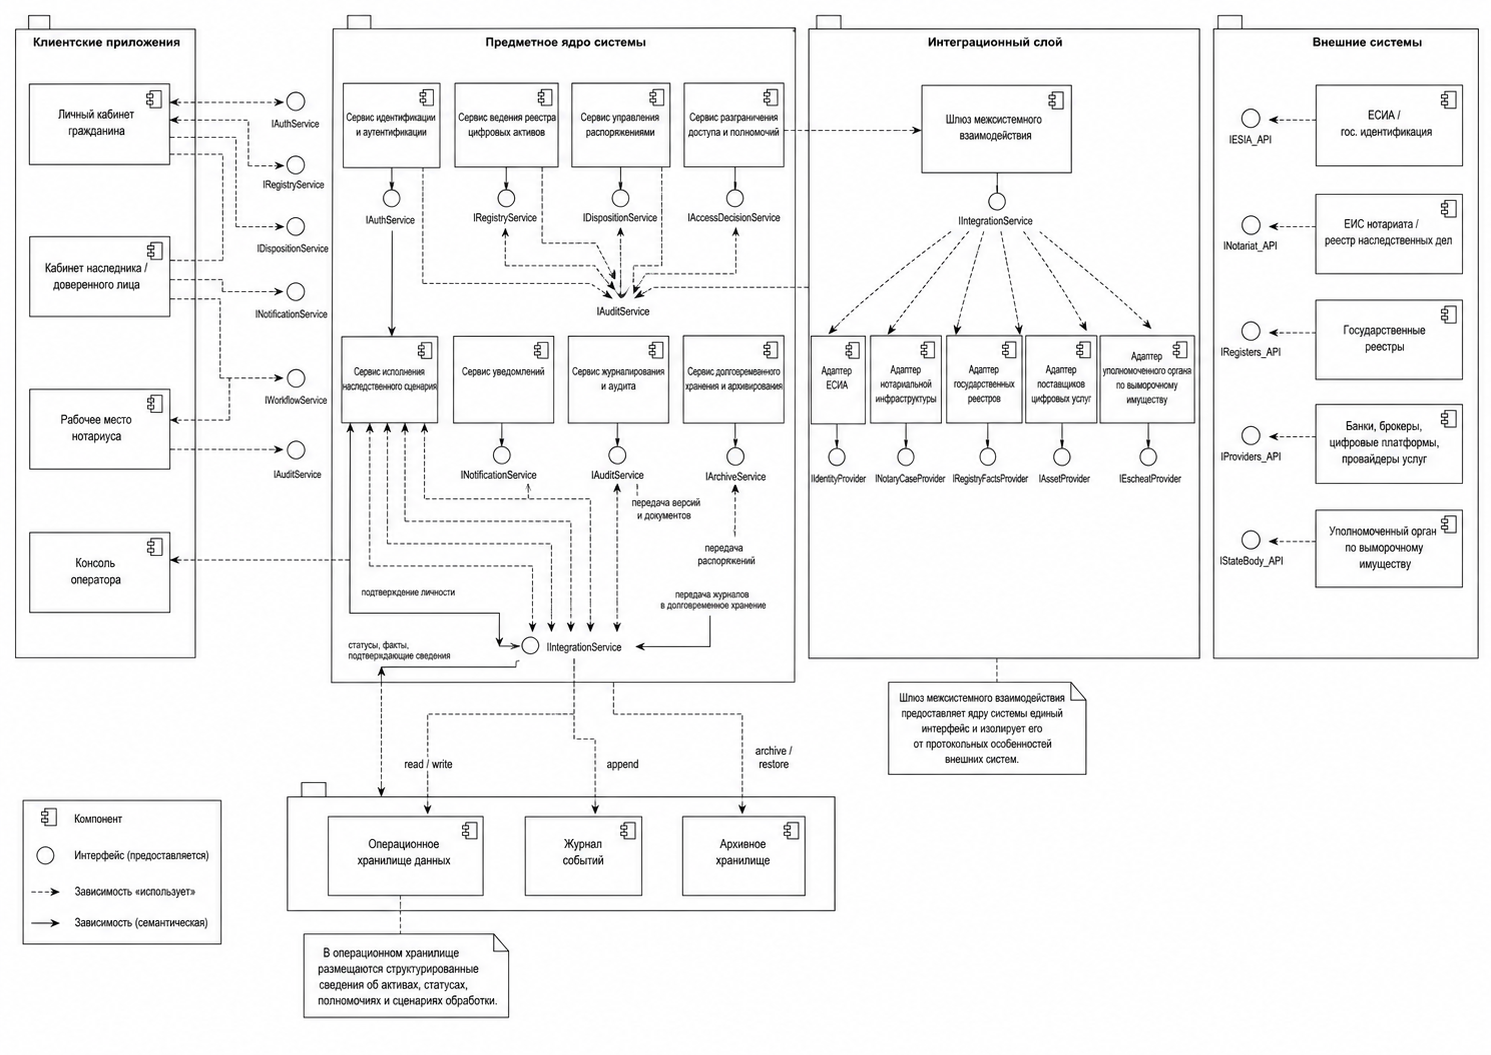
\includegraphics[width=\linewidth,height=0.72\textheight,keepaspectratio]{architect.png}
    \caption{Компонентная архитектура государственной информационной системы}
  \end{figure}
\end{frame}

\begin{frame}{Ключевые проектные решения}
  \footnotesize
  \begin{itemize}
    \smallitem
    \item \textbf{Предметное ядро}: реестр активов, управление распоряжениями, наследственный сценарий, разграничение доступа, аудит, архивирование и уведомления.
    \item \textbf{Интеграционный слой}: единый шлюз и адаптеры для ЕСИА, государственных реестров, нотариальной инфраструктуры, поставщиков цифровых услуг и уполномоченного органа по выморочному имуществу.
    \item \textbf{Разделение хранилищ}: операционные данные, журнал событий, архивное хранилище и защищённое хранилище контейнеров имеют разные режимы доступа.
    \item \textbf{Защита секретов}: секреты шифруются на клиентской стороне, раскрытие строится на составных ключах и не может выполняться единолично оператором системы.
  \end{itemize}
\end{frame}

\begin{frame}{Технико-экономическое обоснование}
  \scriptsize
  \begin{table}
    \centering
    \begin{tabular}{L{0.45\linewidth} C{0.22\linewidth} C{0.16\linewidth}}
      \toprule
      \textbf{Показатель} & \textbf{Значение} & \textbf{Период} \\
      \midrule
      Труд проектной команды & 102,739 млн руб. & 18 месяцев \\
      Накладные расходы & 15,411 млн руб. & проект \\
      Инфраструктура первой очереди & 22,000 млн руб. & проект \\
      Внедрение, документация, обучение & 12,000 млн руб. & проект \\
      Аудит безопасности и пилот защищённого хранения & 10,500 млн руб. & проект \\
      Резерв проектных рисков & 16,265 млн руб. & проект \\
      \midrule
      \textbf{Единовременные затраты первой очереди} & \textbf{178,915 млн руб.} & \textbf{проект} \\
      \textbf{Годовые эксплуатационные затраты} & \textbf{56,251 млн руб.} & \textbf{год} \\
      \bottomrule
    \end{tabular}
  \end{table}
\end{frame}

\begin{frame}{Экономический эффект}
  \scriptsize
  \begin{columns}[T,onlytextwidth]
    \begin{column}{0.43\linewidth}
      \begin{block}{Прямой эффект}
        \metric{120 млн руб./год}{снижение трудозатрат и административных расходов}
        \vspace{0.2cm}

        \metric{63,75 млн руб./год}{чистый прямой эффект после эксплуатационных затрат}
        \vspace{0.2cm}

        \metric{2,81 года}{срок компенсации единовременных затрат по прямому эффекту}
      \end{block}
      \begin{block}{С учётом расширенного хранения}
        \metric{79,75 млн руб./год}{совокупный чистый эффект}
        \vspace{0.2cm}

        \metric{2,24 года}{расчётный срок компенсации затрат}
      \end{block}
    \end{column}
    \begin{column}{0.55\linewidth}
      \begin{figure}
        \centering
        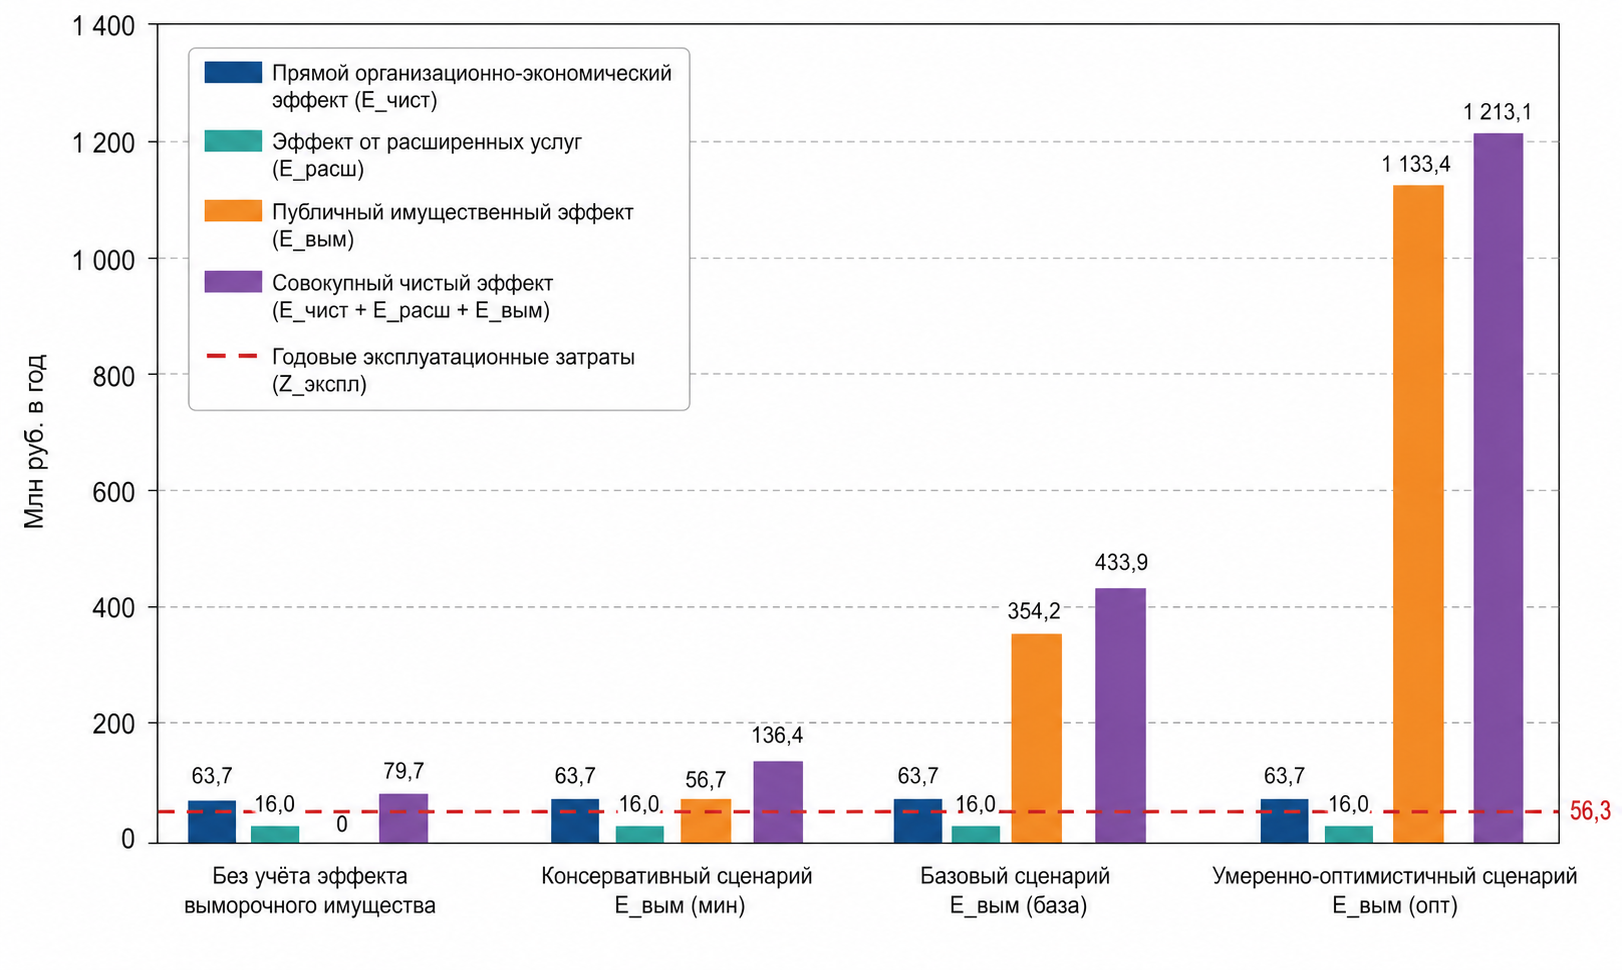
\includegraphics[width=\linewidth,height=0.72\textheight,keepaspectratio]{economic.png}
        \caption{Сценарная оценка годового экономического эффекта внедрения}
      \end{figure}
    \end{column}
  \end{columns}
\end{frame}

\begin{frame}{Основные результаты работы}
  \footnotesize
  \begin{enumerate}
    \smallitem
    \item Проведён анализ теоретических, правовых и методических основ управления цифровыми активами граждан; выявлены ключевые риски хранения, передачи и наследования.
    \item Определены участники процесса, целевой сценарий работы системы, а также функциональные и нефункциональные требования к государственной информационной системе.
    \item Разработано концептуальное проектное решение: архитектура, состав подсистем, интеграционный контур, подход к защищённому хранению и юридически значимому аудиту.
    \item Выполнена укрупнённая оценка затрат и экономического эффекта: проект экономически обоснован за счёт сокращения трудоёмкости, компенсации части затрат расширенными услугами и повышения полноты выявления цифрово фиксируемых активов.
  \end{enumerate}
\end{frame}

\begin{frame}{Практическая значимость}
  \footnotesize
  \begin{itemize}
    \smallitem
    \item Для граждан: фиксация воли владельца и снижение риска утраты цифровых активов.
    \item Для наследников и доверенных лиц: понятный порядок получения допустимых сведений без произвольного доступа к частной жизни.
    \item Для нотариата: структурированные сведения об активах и распоряжениях в рамках наследственного дела.
    \item Для государства: повышение полноты учёта цифрово фиксируемых активов, включая сценарии выморочного имущества.
    \item Для последующего проектирования: сформирован набор требований, который может быть детализирован в техническое задание, модель данных, модель угроз и регламенты эксплуатации.
  \end{itemize}
\end{frame}

\begin{frame}[plain]
  \centering
  \vspace{1.2cm}
  {\Huge Спасибо за внимание}

  \vspace{0.8cm}
  {\Large Вопросы}
\end{frame}

\end{document}
